%%
%% Beginning of file 'sample61.tex'
%%
%% Modified 2016 September
%%
%% This is a sample manuscript marked up using the
%% AASTeX v6.1 LaTeX 2e macros.
%%
%% AASTeX is now based on Alexey Vikhlinin's emulateapj.cls 
%% (Copyright 2000-2015).  See the classfile for details.

%% AASTeX requires revtex4-1.cls (http://publish.aps.org/revtex4/) and
%% other external packages (latexsym, graphicx, amssymb, longtable, and epsf).
%% All of these external packages should already be present in the modern TeX 
%% distributions.  If not they can also be obtained at www.ctan.org.

%% The first piece of markup in an AASTeX v6.x document is the \documentclass
%% command. LaTeX will ignore any data that comes before this command. The 
%% documentclass can take an optional argument to modify the output style.
%% The command below calls the preprint style  which will produce a tightly 
%% typeset, one-column, single-spaced document.  It is the default and thus
%% does not need to be explicitly stated.
%%
%%
%% using aastex version 6.1
\documentclass[twocolumn]{aastex62}

%% The default is a single spaced, 10 point font, single spaced article.
%% There are 5 other style options available via an optional argument. They
%% can be envoked like this:
%%
%% \documentclass[argument]{aastex61}
%% 
%% where the arguement options are:
%%
%%  twocolumn   : two text columns, 10 point font, single spaced article.
%%                This is the most compact and represent the final published
%%                derived PDF copy of the accepted manuscript from the publisher
%%  manuscript  : one text column, 12 point font, double spaced article.
%%  preprint    : one text column, 12 point font, single spaced article.  
%%  preprint2   : two text columns, 12 point font, single spaced article.
%%  modern      : a stylish, single text column, 12 point font, article with
%% 		  wider left and right margins. This uses the Daniel
%% 		  Foreman-Mackey and David Hogg design.
%%
%% Note that you can submit to the AAS Journals in any of these 6 styles.
%%
%% There are other optional arguments one can envoke to allow other stylistic
%% actions. The available options are:
%%
%%  astrosymb    : Loads Astrosymb font and define \astrocommands. 
%%  tighten      : Makes baselineskip slightly smaller, only works with 
%%                 the twocolumn substyle.
%%  times        : uses times font instead of the default
%%  linenumbers  : turn on lineno package.
%%  trackchanges : required to see the revision mark up and print its output
%%  longauthor   : Do not use the more compressed footnote style (default) for 
%%                 the author/collaboration/affiliations. Instead print all
%%                 affiliation information after each name. Creates a much
%%                 long author list but may be desirable for short author papers
%%
%% these can be used in any combination, e.g.
%%
%% \documentclass[twocolumn,linenumbers,trackchanges]{aastex61}

%% AASTeX v6.* now includes \hyperref support. While we have built in specific
%% defaults into the classfile you can manually override them with the
%% \hypersetup command. For example,
%%
%%\hypersetup{linkcolor=red,citecolor=green,filecolor=cyan,urlcolor=magenta}
%%
%% will change the color of the internal links to red, the links to the
%% bibliography to green, the file links to cyan, and the external links to
%% magenta. Additional information on \hyperref options can be found here:
%% https://www.tug.org/applications/hyperref/manual.html#x1-40003

%% If you want to create your own macros, you can do so
%% using \newcommand. Your macros should appear before
%% the \begin{document} command.
%%
\usepackage{multirow}
\newcommand{\vdag}{(v)^\dagger}
\newcommand\aastex{AAS\TeX}
\newcommand\latex{La\TeX}
\newcommand{\sm}{M_\odot}
\newcommand{\sr}{R_\odot}

%% Reintroduced the \received and \accepted commands from AASTeX v5.2
\received{\today}
\revised{}
\accepted{}
%% Command to document which AAS Journal the manuscript was submitted to.
%% Adds "Submitted to " the arguement.
\submitjournal{PASP}

%% Mark up commands to limit the number of authors on the front page.
%% Note that in AASTeX v6.1 a \collaboration call (see below) counts as
%% an author in this case.
%
%\AuthorCollaborationLimit=3
%
%% Will only show Schwarz, Muench and "the AAS Journals Data Scientist 
%% collaboration" on the front page of this example manuscript.
%%
%% Note that all of the author will be shown in the published article.
%% This feature is meant to be used prior to acceptance to make the
%% front end of a long author article more manageable. Please do not use
%% this functionality for manuscripts with less than 20 authors. Conversely,
%% please do use this when the number of authors exceeds 40.
%%
%% Use \allauthors at the manuscript end to show the full author list.
%% This command should only be used with \AuthorCollaborationLimit is used.

%% The following command can be used to set the latex table counters.  It
%% is needed in this document because it uses a mix of latex tabular and
%% AASTeX deluxetables.  In general it should not be needed.
%\setcounter{table}{1}

%%%%%%%%%%%%%%%%%%%%%%%%%%%%%%%%%%%%%%%%%%%%%%%%%%%%%%%%%%%%%%%%%%%%%%%%%%%%%%%%
%%
%% The following section outlines numerous optional output that
%% can be displayed in the front matter or as running meta-data.
%%
%% If you wish, you may supply running head information, although
%% this information may be modified by the editorial offices.
\shorttitle{PS1 Star-galaxy Catalog}
\shortauthors{One then the other}
%%
%% You can add a light gray and diagonal water-mark to the first page 
%% with this command:
\watermark{DRAFT}
%% where "text", e.g. DRAFT, is the text to appear.  If the text is 
%% long you can control the water-mark size with:
%  \setwatermarkfontsize{dimension}
%% where dimension is any recognized LaTeX dimension, e.g. pt, in, etc.
%%
%%%%%%%%%%%%%%%%%%%%%%%%%%%%%%%%%%%%%%%%%%%%%%%%%%%%%%%%%%%%%%%%%%%%%%%%%%%%%%%%

%%%%%%%%%%%%%%%%%%%%%%%%%%%%%%%%%%%%%%%%%%%%%%%%%%%%%%%%%%%%%%%%%%%%%%%%%%%%%%%%
%%
%% The following section defines new commands for comments from co-authors
%%
\newcommand{\yutaro}[1]{{\color{red} yt: {#1}}}
\newcommand{\NC}[1]{{\color{brown} NC: {#1}}}
\newcommand{\aam}[1]{{\color{blue} aam: {#1}}}
\newcommand{\todo}[1]{{\color{magenta} to-do: {#1}}}
%%
%%%%%%%%%%%%%%%%%%%%%%%%%%%%%%%%%%%%%%%%%%%%%%%%%%%%%%%%%%%%%%%%%%%%%%%%%%%%%%%%

%% This is the end of the preamble.  Indicate the beginning of the
%% manuscript itself with \begin{document}.

\begin{document}

\title{\textbf{something better needed} A Machine Learning Model to Separate Stars and Galaxies in PanSTARRS1 Data}

%% LaTeX will automatically break titles if they run longer than
%% one line. However, you may use \\ to force a line break if
%% you desire. In v6.1 you can include a footnote in the title.

%% A significant change from earlier AASTEX versions is in the structure for 
%% calling author and affilations. The change was necessary to implement 
%% autoindexing of affilations which prior was a manual process that could 
%% easily be tedious in large author manuscripts.
%%
%% The \author command is the same as before except it now takes an optional
%% arguement which is the 16 digit ORCID. The syntax is:
%% \author[xxxx-xxxx-xxxx-xxxx]{Author Name}
%%
%% This will hyperlink the author name to the author's ORCID page. Note that
%% during compilation, LaTeX will do some limited checking of the format of
%% the ID to make sure it is valid.
%%
%% Use \affiliation for affiliation information. The old \affil is now aliased
%% to \affiliation. AASTeX v6.1 will automatically index these in the header.
%% When a duplicate is found its index will be the same as its previous entry.
%%
%% Note that \altaffilmark and \altaffiltext have been removed and thus 
%% can not be used to document secondary affiliations. If they are used latex
%% will issue a specific error message and quit. Please use multiple 
%% \affiliation calls for to document more than one affiliation.
%%
%% The new \altaffiliation can be used to indicate some secondary information
%% such as fellowships. This command produces a non-numeric footnote that is
%% set away from the numeric \affiliation footnotes.  NOTE that if an
%% \altaffiliation command is used it must come BEFORE the \affiliation call,
%% right after the \author command, in order to place the footnotes in
%% the proper location.
%%
%% Use \email to set provide email addresses. Each \email will appear on its
%% own line so you can put multiple email address in one \email call. A new
%% \correspondingauthor command is available in V6.1 to identify the
%% corresponding author of the manuscript. It is the author's responsibility
%% to make sure this name is also in the author list.
%%
%% While authors can be grouped inside the same \author and \affiliation
%% commands it is better to have a single author for each. This allows for
%% one to exploit all the new benefits and should make book-keeping easier.
%%
%% If done correctly the peer review system will be able to
%% automatically put the author and affiliation information from the manuscript
%% and save the corresponding author the trouble of entering it by hand.

\correspondingauthor{A.~A.~Miller}
\email{amiller@northestern.edu}

% \author[0000-0001-9515-478X]{A.~A.~Miller}
% \affil{Center for Interdisciplinary Exploration and Research in Astrophysics (CIERA) and Department of Physics and Astronomy, Northwestern University, 2145 Sheridan Road, Evanston, IL 60208, USA}
% \affil{The Adler Planetarium, Chicago, IL 60605, USA}

\author{Concerned ZTF Scientists}
\affil{Zwicky Transient Facility}

%% Note that the \and command from previous versions of AASTeX is now
%% depreciated in this version as it is no longer necessary. AASTeX 
%% automatically takes care of all commas and "and"s between authors names.

%% AASTeX 6.1 has the new \collaboration and \nocollaboration commands to
%% provide the collaboration status of a group of authors. These commands 
%% can be used either before or after the list of corresponding authors. The
%% argument for \collaboration is the collaboration identifier. Authors are
%% encouraged to surround collaboration identifiers with ()s. The 
%% \nocollaboration command takes no argument and exists to indicate that
%% the nearby authors are not part of surrounding collaborations.

%% Mark off the abstract in the ``abstract'' environment. 
\begin{abstract}

We did a decent job of separating stars and galaxies.

\end{abstract}

%% Keywords should appear after the \end{abstract} command. 
%% See the online documentation for the full list of available subject
%% keywords and the rules for their use.
\keywords{catalogs --- galaxies: statistics --- methods: data analysis --- methods: statistical --- stars: statistics --- surveys}

%% From the front matter, we move on to the body of the paper.
%% Sections are demarcated by \section and \subsection, respectively.
%% Observe the use of the LaTeX \label
%% command after the \subsection to give a symbolic KEY to the
%% subsection for cross-referencing in a \ref command.
%% You can use LaTeX's \ref and \label commands to keep track of
%% cross-references to sections, equations, tables, and figures.
%% That way, if you change the order of any elements, LaTeX will
%% automatically renumber them.

%% We recommend that authors also use the natbib \citep
%% and \citet commands to identify citations.  The citations are
%% tied to the reference list via symbolic KEYs. The KEY corresponds
%% to the KEY in the \bibitem in the reference list below. 

\section{Introduction}\label{sec:intro}

\NC{
To develop the star/galaxy classifier applicable for any variable sources detected by ZTF project, 
the wide-field 3$\pi$ Pan-STARRS1 (PS1) survey \citep{Chambers16} 
would provide the most felicitous data set. 

The PS1 survey uses a wide-field f/4.4 optical telescope system 
at the Haleakala Observatory on the island of Maui in Hawaii. 
The system comprises a 1.8 m primary and 0.9 m secondary mirrors \citep{Hodapp04}, 
produces a field of view of 3.3 deg$^2$ with 60 CCD chips each of 4800$\times$4800 pixels, 
and the pixel resolution is 0.258 arcsec pixel$^{-1}$ at the focal plane. 
The filter system consists of five main broadband filters, 
$g_{\mathrm{P1}}$, $r_{\mathrm{P1}}$, $i_{\mathrm{P1}}$, $z_{\mathrm{P1}}$, and $y_{\mathrm{P1}}$, 
and that effective wavelength is 481 nm, 617 nm, 752 nm, 866 nm, and 962 nm, 
respectively \citep{Tonry12, Schlafly12}. 
The typical 5$\sigma$ depth of stack image is 23.3, 23.2, 23.1, 22.3, and 21.3 mag 
white that of a single epoch is 22.0, 21.8, 21.5, 20.9, and 19.7 mag in the AB system, 
with a median seeing of 1.31, 1.19, 1.11, 1.07, and 1.02 arcsec, respectively \citep{Chambers16}. 

The first Pan-STARRS data release (DR1) provides the pixel-based shape measurements 
({\it e.g.,} the half radial moment \texttt{momentRH}, the major axis of FWHM \texttt{psfMajorFWHM}; 
\citealt{Flewelling16}) 
for $>$3 billion sources based off of the stack images in the five filters \citep{Magnier16b}, 
using the imaging data from 3$\pi$ survey ($\mathrm{Decl.}>-30\ \mathrm{deg}$) 
carried out several times per filter and over a four-year time span. 




}

\yutaro{define features}

\section{Model Data}\label{sec:model_data}

Data for the star-galaxy model were obtained from the PS1 casjobs
server.\footnote{http://mastweb.stsci.edu/ps1casjobs/home.aspx} The PS1
database provides flux measurements via aperture photometry,
point-spread-function (PSF) photometry, and \citet{Kron80}
photometry.\footnote{A subset of bright sources ($i < 21\,\mathrm{mag}$)
outside the Galactic plane have additional photometric measurements, e.g.,
exponential or \citet{Sersic63} profiles, in the \textit{StackModelFitExp} and
\textit{StackModelFitSer} tables, respectively. We ignore these measurements
for this study as they are not available for all sources.} These flux
measurements are produced by PS1 in 3 different ways. The mean brightness
measured on the individual PS1 frames is reported in the \textit{MeanObject}
table, the mean brightness measured via forced-PSF/aperture photometry on the
individual PS1 frames is reported in the \textit{ForcedMeanObject} table, and
finally, the brightness measured on the full-depth stacked PS1 images is
reported in the \textit{StackObjectThin} table. The
\textit{StackObjectAttributes} table further supplements these tables with
point-source object shape measurements, which are very useful to discriminate
stars and galaxies. Ultimately, see \S\ref{sec:simple_model}, we use flux
measurements from the \textit{StackObjectThin} table and shape measurements
from the \textit{StackObjectAttributes} to build our models.


\subsection{The SDSS Training Set}\label{sec:sdss}

\todo{Need to explain why we use the HST set to train the model}

\begin{figure*}[t]
 \centering
  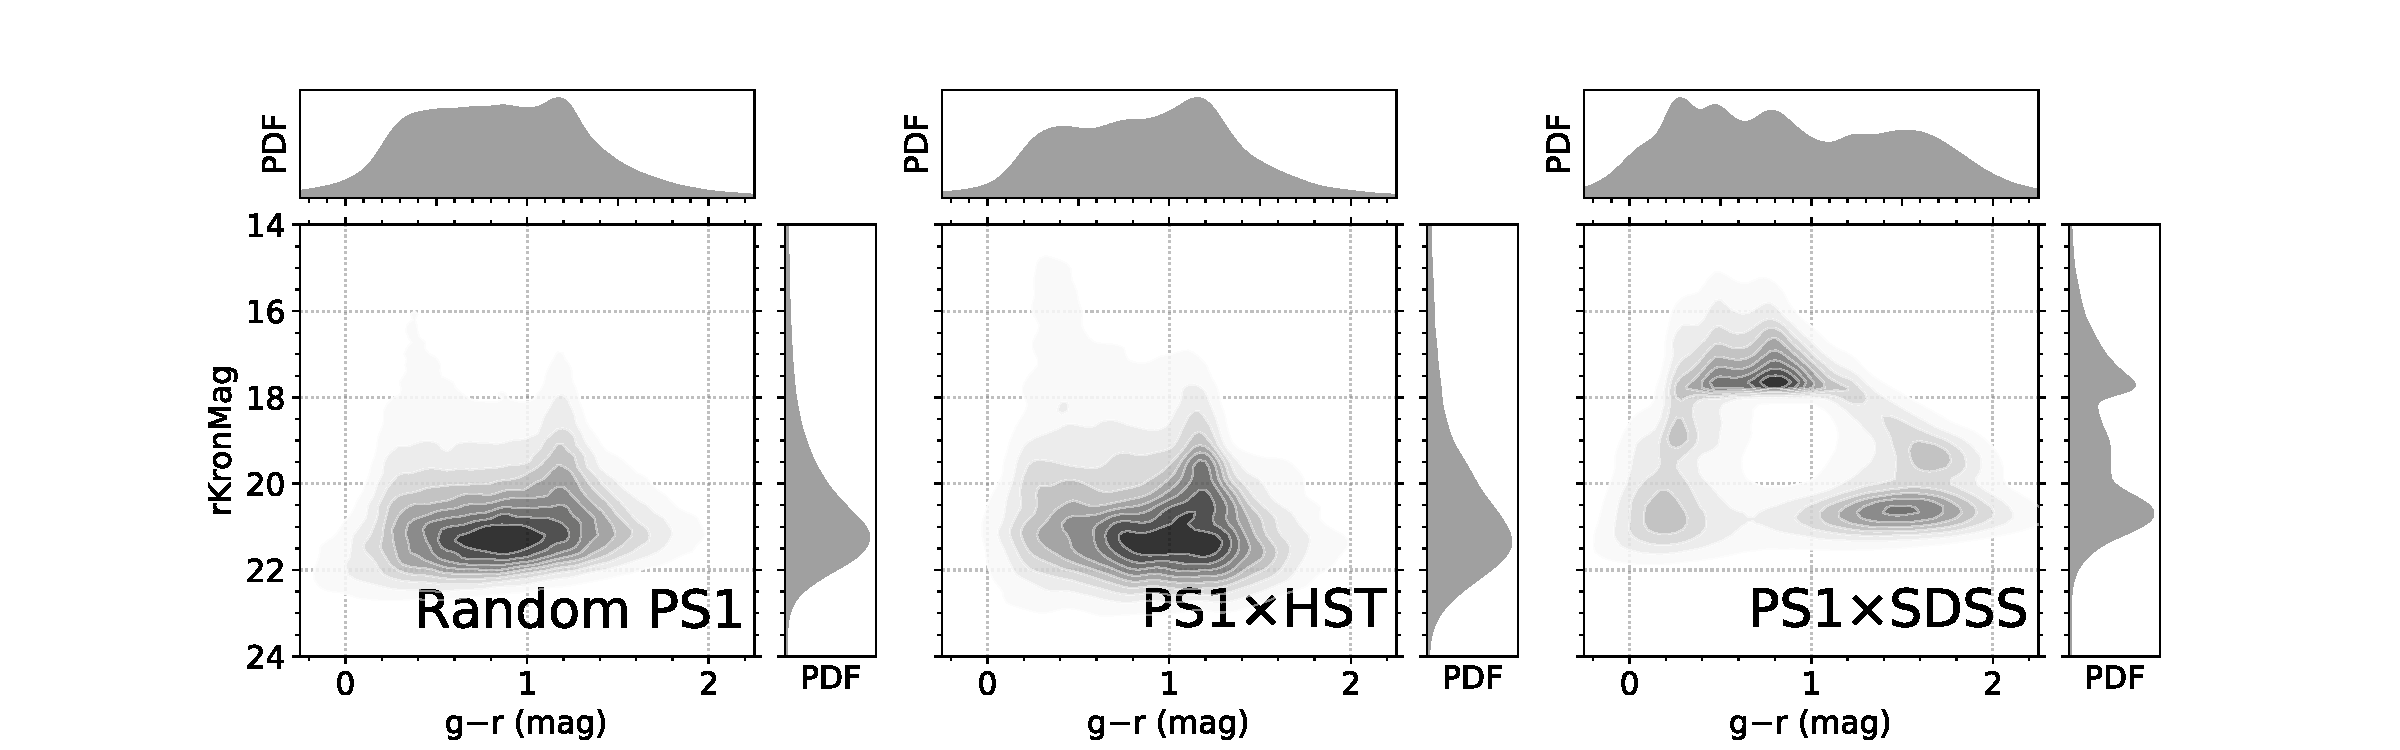
\includegraphics[width=7in, bb = 79 3 1061 333]{./Figures/ColorMagDiagramComb.pdf}
  \caption{
  \NC{
  Color magnitude diagrams (CMDs) for sources in the PS1 catalog selected through three different procedures. 
  From left to right, we show a KDE of the PDF of the CMD for randomly selected 1M PS1 sources, 
  PS1 sources cross-matched against the HST COSMOS sources, 
  and those against the SDSS spectroscopic sources. 
  The population density is represented as grayscale colormap, 
  and white lines on the KDE show contours of it at from 0.1 to 1.0 by 0.1 interval. 
  A KDE of the PDF of the color ($\mathrm{gKronMag} - \mathrm{rKronMag}$) and \texttt{rKornMag} 
  is also shown in the upper side and the left side of the CMD for each data set. 
  }
  }
  %
  \label{fig:cmd}
\end{figure*}

\subsection{The \textit{HST} Training Set} 

A fundamental challenge in the construction of any supervised machine learning
model is the curation of a high-fidelity training set. A subset of the data
that requires classification must have known labels so the machine can learn
the proper mapping between features and labels. The superior image quality of
the \textit{Hubble Space Telescope} (\textit{HST}) provides exceptionally
accurate morphological classifications, making it an ideal source of a training
set for lower quality ground-based imaging (e.g., \citealt{Lupton01}). The
downside of \textit{HST} is that the field of view is relatively small, so it
is difficult to construct a large and diverse training set suitable for
predictions over the entire sky.

We use the largest contiguous area imaged by \textit{HST}, the 1.64\,deg$^2$
COSMOS field, to construct a training set for our models. Morphological
classifications of \textit{HST} COSMOS sources are provided in
\citet{Leauthaud07}. \citeauthor{Leauthaud07} demonstrate reliable
classifications down to $\sim$25\,mag, which is significantly deeper than the
faintest sources detected by PS1. We identify counterparts in the PS1 and
\textit{HST} data by performing a spatial crossmatch between the two catalogs
using a 1\arcsec radius.\footnote{This matching radius is the same employed by
PS1 to associate individual detections in the \textit{MeanObject} table with
detections in the \textit{StackObjectAttributes} table.} We further excluded
sources from the \citet{Leauthaud07} catalog with $\texttt{MAG\_AUTO} >
25$\,mag, as these sources are too faint to be detected by PS1 meaning their
crossmatch counterparts are likely spurious. Following this procedure, we find
that there are 87,431 sources in the \citet{Leauthaud07} catalog with PS1
counterparts. Of these, 80,974 are unique in that there is a one-to-one
correspondence between \textit{HST} source and a single PS1 \textit{ObjID}. The
training set is further reduced to 75,927 once our detection criteria are
applied (see \S\ref{sec:simple_model}), and, of those, only 47,093 have
$\texttt{nDetections} \ge 1$ in the PS1
database.\footnote{$\texttt{nDetections}$ refers to the number of detections in
individual PS1 exposures. Thus, \textit{StackObjectThin} souces can have
$\texttt{nDetections}$ = 0 if the source is only detected in the PS1 stack
images.}

\todo{Is there an interesting figure to show here that isn't redundant with other figures that we will show?}

\section{Model Features}\label{sec:model_features}

In addition to developing a training set, we must select features to use as an input for the model. As noted in \S\ref{sec:model_data}, the PS1 database provides flux and shape measurements in each of the $grizy$ filters. Adopting each of these measurements as features for the model presents a significant problem: missing data. There are relatively few sources in the PS1 database that are detected in all 5 filters. There are two general solutions to this problem: (i) remove sources detected in fewer than 5 filters, or (ii) assign some value, via either imputation (e.g., \citealt{Miller17}) or the use of a dummy variable, to the missing data. Given that the vast majority of PS1 sources are faint and are not detected in all 5 filters, neither of these possiblities is attractive for our present purposes.

Rather than use the raw features from the database, we engineer a series of ``white flux'' features that combine the relevant measurements across all filters in which a source is detected. In a given filter, a source is detected if the $\mathtt{PSFFlux}_f$, $\mathtt{KronFlux}_f$, and $\mathtt{ApFlux}_f$ are \textit{all $> 0$}, where the $f$ subscript refers to a specific filter. The ``white flux'' feature is then created as:
%
\begin{equation}
    \mathtt{white[Feat]} =  \frac{\sum_f^{f = grizy} w_f  \, \mathtt{Feat}_f \, \mathrm{det}_f}{\sum_f^{f = grizy} w_f}, 
\end{equation}
%
where the sum is over all 5 PS1 filters, \texttt{Feat} is the feature from the \textit{StackObjectAttributes} table, $\mathrm{det}_f = 1$ if the source is detected in the $f$ filter, as defined above, or $\mathrm{det}_f = 0$ if not detected, and $w_f$ is the weight assigned to each filter:
%
\begin{equation}
    w_f = \left(\frac{\mathtt{KronFlux}_f}{\mathtt{KronFluxErr}_f}\right)^2,
\end{equation}
%
equivalent to signal-to-noise ratio (SNR) squared in the given filter. Ultimately, the ``white flux'' features correspond to a weighted mean, with weights equal to the square of the SNR. 

Our final model includes 11 ``white flux'' features to separate stars and galaxies. The database features include: \texttt{PSFFlux}\footnote{For the \texttt{PSFFlux} feature $w_f = (\mathtt{PSFFlux}_f/\mathtt{PSFFluxErr}_f)^2$.}, \texttt{KronFlux}, \texttt{ApFlux}\footnote{For the \texttt{ApFlux} feature $w_f = (\mathtt{ApFlux}_f/\mathtt{ApFluxErr}_f)^2$.}, \texttt{ExtNSigma}, \texttt{KronRad}, \texttt{psfChiSq}, \texttt{psfLikelihood}, \texttt{momentYY}, \texttt{momentXY}, \texttt{momentXX}, and \texttt{momentRH}\footnote{\NC{We normalized the shape measurements using the average of \texttt{psfMajorFWHM} and  \texttt{psfMinorFWHM} before utilizing them for training the classifier. }}. The remaining features in the database were either uninformative or would bias the model, such as R.A.\ and Dec.\ (see e.g., \citealt{Richards12a,Miller17}). We do not directly include \texttt{whitePSFFlux}, \texttt{whiteKronFlux}, and \texttt{whiteApFlux} in the model. We found that the inclusion of these features resulted in a bias whereby all sources brighter than $\sim$16\,mag were automatically classified as stars. Instead, we include the ratio of the different flux measures: \texttt{whitePSFKronRatio} = \texttt{whitePSFFlux}/\texttt{whiteKronFlux}, \texttt{whitePSFApRatio} = \texttt{whitePSFFlux}/\texttt{whiteApFlux}, as well as a third feature \texttt{whitePSFKronDist} (see \S\ref{sec:simple_model}).

As we previously alluded to, the primary benefit of the ``white flux'' features is that they can be calculated for every source in PS1 thus allowing each to be compared on common ground. Furthermore, the SNR for the ``white flux'' features is greater than the SNR for the equivalent feature in a single filter. The downside of these features is that for some sources, especially at the bright end, color information is lost. While a blue source and red source with identical \texttt{whitePSFFlux} values are intrinsically very different, the ``white flux'' features obscure that information for the classifier. Ultimately, we tested models with and without the ``white flux'' features and found that models using only the ``white flux'' features outperform those that do not. We conclude that the benefits of this approach outweigh any loss of color information. 

\begin{figure}[t]
 \centering
  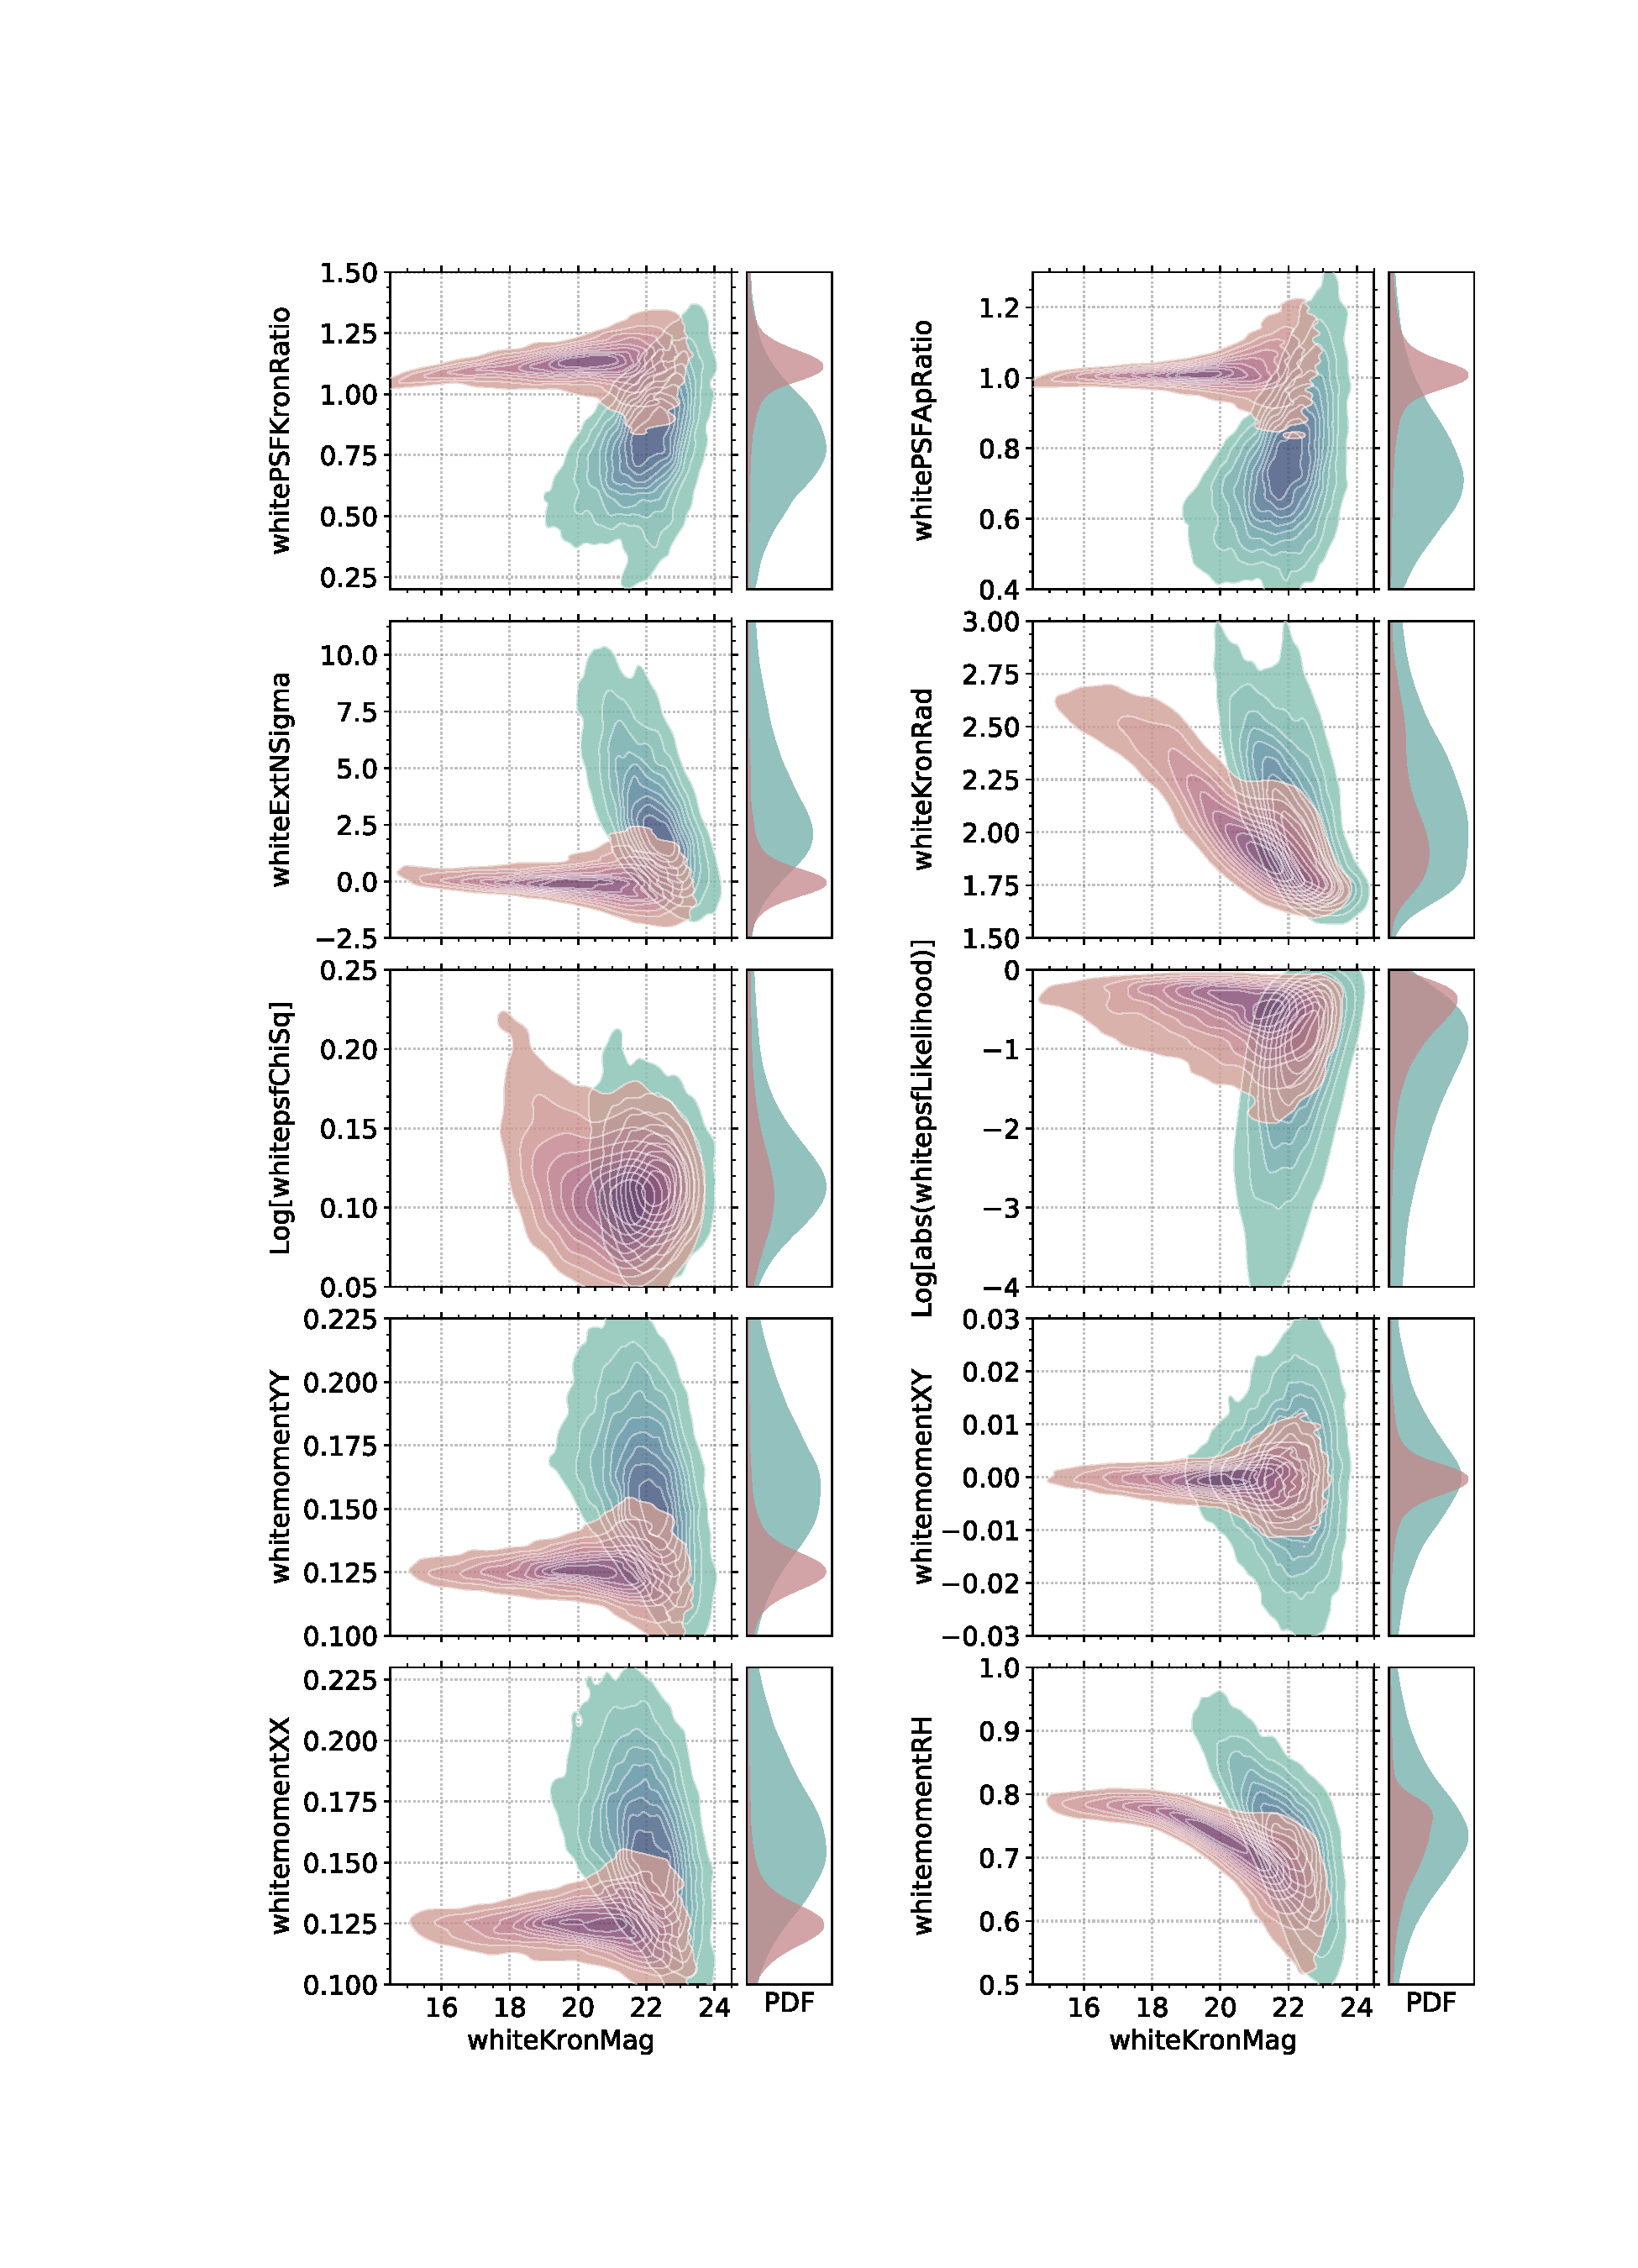
\includegraphics[width=3.5in, bb = 139 113 862 1163]{./Figures/whiteFeatures.pdf}
  \caption{
  \NC{KDE of the PDF for white features as a function of \texttt{whiteKronMag}
  ($=-2.5\log_{10}[\mathtt{whiteKronFlux}/3631]$) 
  for all PS1 sources with HST classification. 
  The population density for stars and galaxies of each feature is represented by the depth of red and green, respectively, 
  and white lines on them show the contours of the population density at from 0.1 to 1.0 by an interval of 0.1.
  The density is scaled relative to the total number of stars and galaxies in the dataset we used for the training of the ML model. 
  The differing PSDs for the two populations ({\textit i.e.,} stars and galaxies) suggest that 
  the machine learning method capturing non-linear behavior in multidimensional features 
  may produce a significant improvement over both of the PS1 model and the simple model. }
  }
  %
  \label{fig:features}
\end{figure}

The distribution of ``white flux'' features for stars and galaxies in the \textit{HST} training set is shown in Figure~\ref{fig:features} (\texttt{whitePSFKronDist} is shown in Figure~\ref{fig:psfkrondist}). As might be expected, it is clear from Figure~\ref{fig:features} that stars and galaxies are easily separated at the bright end ($\lesssim 20$\,mag), but there is significant overlap in the featurespace between the two populations at the faint end ($\sim$23\,mag). Machine learning algorithms are capable of capturing non-linear behavior in multidimentional data sets, which will prove especially useful for the sources under consideration in the PS1 data set. 



\section{Model Construction}
\subsection{The PS1 Baseline Model}\label{sec:ps1_model}

To establish a baseline for the performance of our star-galaxy separation models we adopt the classification criteria in the PS1 documentation, namely sources with
$$ \mathtt{iPSFMag} - \mathtt{iKronMag} > 0.05\;\mathrm{mag},$$
are classified as galaxies.\footnote{\url{https://outerspace.stsci.edu/display/PANSTARRS/How+to+separate+stars+and+galaxies}} The documentation notes that this classification can be performed using photometry from any of the \textit{MeanObject}, \textit{ForcedMeanObject}, or \textit{StackedObjectThin} tables. The PS1 documentation further notes that this basic cut does not perform well for sources with $i \gtrsim 21\,\mathrm{mag}$, which constitutes the majority of sources detected by PS1, and motivates us to generate our own star-galaxy separation models. We use the performance of the $\mathtt{iPSFMag} - \mathtt{iKronMag} > 0.05\;\mathrm{mag}$ model (hereafter, the PS1 model) as a baseline to compare to the models discussed below.

\subsection{Simple Model}\label{sec:simple_model}

While our ultimate goal is to build a machine learning model to separate stars and galaxies (\S\ref{sec:rf_model}), we first construct a straightforward model. This model is inspired by the SDSS \texttt{photo} pipeline \citep{Lupton01}, and combines the flux in each of the 5 PS1 filters to improve the SNR relative to any individual band. In addition to being easy to interpret, this model (hereafter, the simple model), which utilizes the difference between the PSF flux and the Kron-aperture flux for classification, serves as an additional baseline to test the need for a more complicated machine learning model. 

\NC{
Since only the i-band photometric measurement is used for the star-galaxy separation  
in the PS1 model as explained in \S\ref{sec:simple_model},  
it is expected that the separation accuracy is improved 
by the model with the photometric measurement in all of the five optical bands 
provided by PS1 (g, r, i, z, and y), especially for the source 
detected with a higher signal to noise ratio (S/N) by the other band than that of i-band. 
We therefore created a simple model (hereafter, the simple model) for the separation 
with the photometric measurement in all of the optical bands 
for referring it as a new strict baseline model for the machine learning model  
we developed (described in \S\ref{sec:rf_model}).

The essential idea for the separation by the simple model is the same as the PS1 model;  
sources with a ratio of the $\mathtt{KronFlux}$ to the $\mathtt{PSFFlux}$ 
(corresponding to $\mathtt{PSFMag} - \mathtt{KronMag}$) larger than a threshold 
are classified as galaxies, 
but instead of $\mathtt{i[PSF, Kron]Mag}$,  
we use the white flux measurements ($\mathtt{w[PSF,Kron]Flux}$) 
defined by the weighted average of the flux in all of the optical band:   
$$
\mathtt{w[PSF, Kron]Flux} =  \frac{\sum w_c  F_c }{\sum w_c}, 
\ w_c = \left( \frac{F_c}{e_c} \right)^2, 
$$
where $c = [\mathtt{g, r, i, z, y}]$,  $F$ is the $\mathtt{[PSF,Kron]Flux}$, 
and $e$ is the $\mathtt{[PSF,Kron]FluxErr}$.  
The weight $w = \mathrm{(S/N)}^2$ allows this model to perform better decision 
than the normal average ($w = 1$) by retaining the flux information with high S/N more stronger. 

In order to evaluate the probability of that each source is a star or a galaxy quantitatively, 
we decided to use the orthogonal distance from the threshold line 
($\mathtt{wPSFFlux} = a\times \mathtt{wKronFlux}$) 
on the $\mathtt{wPSFFlux}$-$\mathtt{wKronFlux}$ plane for the simple model:  
$$
\mathtt{wPSFKronDist}(a) = 
	\frac{\mathtt{wPSFFlux} - a\times\mathtt{wKronFlux}}{ \sqrt{1 + a^2}}, 
$$
where $a$ is the critical ratio of the $\mathtt{wPSFFlux}$ to the $\mathtt{wKronFlux}$ 
(corresponding to 0.05 in the PS1 model). 
A bright source, which can be classified clearly, 
has larger $|\mathtt{wPSFKronDist}|$ than that of a faint source, 
even if the ratio of the $\mathtt{wPSFFlux}$ to the $\mathtt{wKronFlux} $
($\propto \mathtt{wPSFMag}  -  \mathtt{wKronMag}$) of them is the same. 
We therefore can use the $\mathtt{wPSFKronDist}$ directly 
as the likelihood of that the source is a star or a galaxy, 
and furthermore, this treatment improves the true positive ratio (TPR) 
at the low false positive ratio (FPR) dramatically (see \S*** and Fig.\ref{fig:cvroc_hst}). 

In this paper, we use $a=0.91375$ derived by the average of $a$ 
through 10-fold cross variation (CV) procedure;   
the data set is split into 10 smaller sets 
and obtain a $a$ by maximizing the TPR at FPR$ = 0.005$ 
(called figure of merit; FoM) of 9 of the folds. 
We repeat this procedure 10 times in total for all of the combination of 9 of the folds. 
The distribution of the $\mathtt{wPSFKronDist}$ on $a=0.91375$ is shown in Fig.\ref{fig:psfkrondist}. 

\begin{figure}[t]
 \centering
  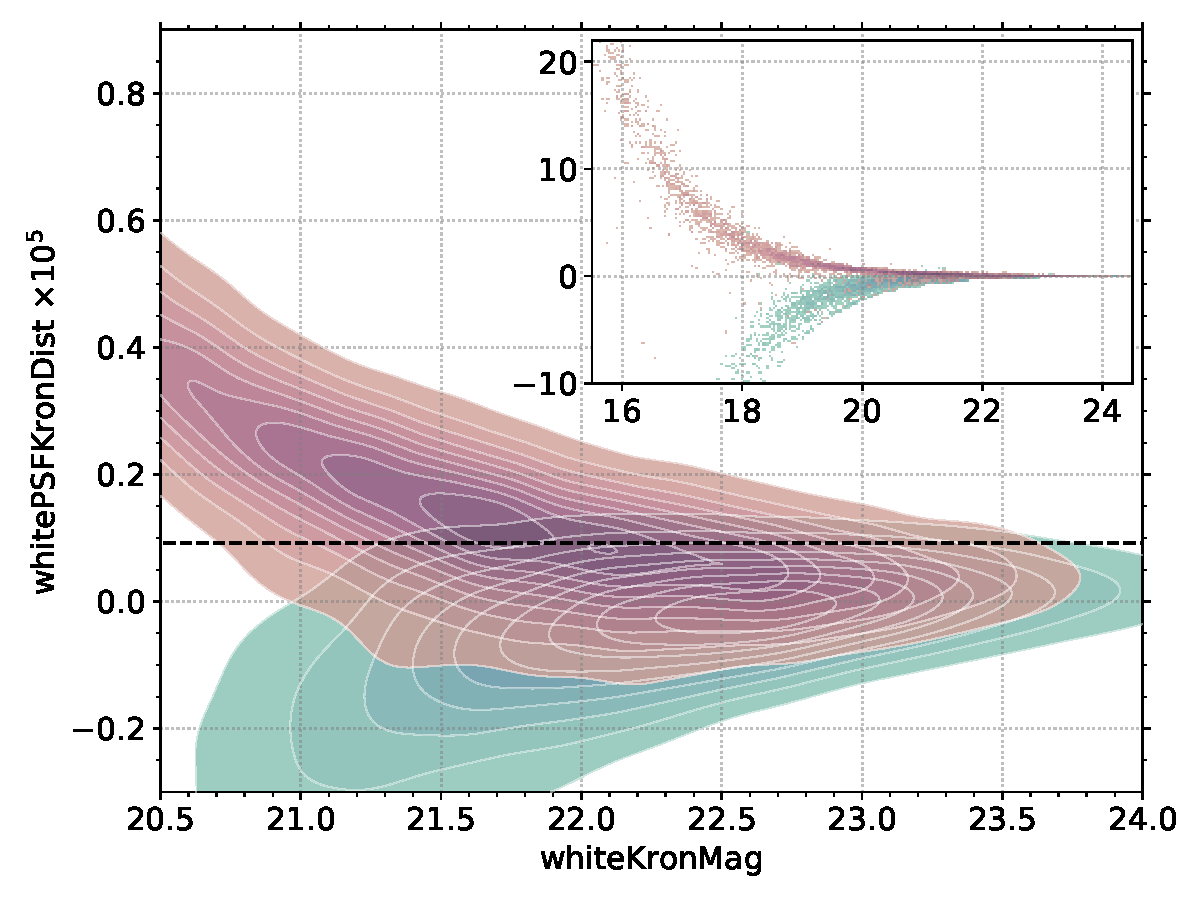
\includegraphics[width=3.35in, bb = 0 0 576 432]{./Figures/whitePSFKronDist.pdf}
  \caption{
  \NC{The distribution of the $\mathtt{wPSFKronDist}$. 
  We show the entire behavior of the $\mathtt{wPSFKronDist}$ for the stars and galaxies 
  in the small window and the KDE of them at the faintest region is shown in the main panel.  
  The dashed line represents the threshold maximizing the separation accuracy for HST sources. }
 }
  %
  \label{fig:psfkrondist}
\end{figure}
}


\subsection{Random Forest Model}\label{sec:rf_model}
\NC{
\subsubsection{The Random Forest Algorithm}\label{sec:rf_alg}
For constructing the machine learning model (hereafter ML model) 
to capture non-linear behavior in multidimensional data sets, 
we use random forest (RF) algorithm in this study.  
This algorithm is based on decision tree models \citep{Quinlan93} 
and bagging, 
wherein bootstrap samples of the training set are used to construct 
each of the $N_{\mathrm{tree}}$ total trees in the forest,
for classification problems \citep{Breiman96, Breiman01}. 
Each tree in the forest is trained by only a random subset of $m_{\mathrm{try}}$ 
features selected from the full feature set, 
and the use of bagging and random selected $m_{\mathrm{try}}$ features 
allows the final model to provide low-bias and low-variance predictions, 
where the number of terminal node (the depth) of individual tree is limited to be larger than \texttt{nodesize}. 

The final predictions for a new unknown source are determined by voting or averaging the predictions 
from each of the individual trees. 
Because of its insensitivity to noisy or meaningless features and also outlier values in them, 
RF algorithms have recently applied for astronomical data sets frequently, 
such as light curve classification ({\it e.g., } \citealt{Richards12a, Huppenkothen17}), 
real and bogus discrimination of difference image ({\it e.g., }  \citealt{Brink13, Wright15}), 
and star and galaxy separation ({\it e.g., } \citealt{Vasconcellos11, Miller17}). 
We utilize the \texttt{Python scikit-learn} implementation of the RF algorithm \citep{Pedregosa12} in this study. 

\subsubsection{Feature Selection}
As we mentioned in \S\ref{sec:model_features}, 11 image features are utilized for training the machine learning classifier: 
\texttt{whiteExtNSigma}, \texttt{whiteKronRad}, \texttt{whitepsfChiSq}, \texttt{whitepsfLikelihood}, 
\texttt{whitemomentYY}, \texttt{whitemomentXY}, \texttt{whitemomentXX}, \texttt{whitemomentRH}, 
\texttt{whitePSFKronRatio}, \texttt{whitePSFApRatio} (Figure \ref{fig:features}), 
and \texttt{whitePSFKronDist} (Figure \ref{fig:psfkrondist}). 

While the ML model trained by RF algorithm 
would provide low-variance and low-biased predictions 
in the presence of strongly correlated features\footnote{Some features have a relatively strong correlation coefficient: 
$\sim0.94$ between \texttt{whiteExtNSigma} and \texttt{whitepsfLikelihood}, 
$\sim0.69$ between \texttt{whiteMomentXX} and \texttt{whiteMomentYY}, and 
$\sim0.50$ between \texttt{whitePSFApRatio} and \texttt{whitePSFKronRatio}. }
 or weak/uninformative features ({\it e.g.,} \citealt{Richards12a}), 
it is worthful to investigate whether the model performance is improved by removing some features. 
We employ two methods to test the full feature set: 
(1) forward feature selection ({\it e.g.,} \citealt{Richards12a, Miller17}) and 
(2) backward feature selection ({\it e.g.,} \citealt{Brink13}). 
In the forward feature selection, 
we construct a series of ML models whereby we iteratively add one feature 
at a time to each successive model starting with the most-important-RF feature 
and ending with the least-important-RF feature 
based on the ranking of \texttt{importance} provided by the RF methods, 
that reflects the contribution of an individual feature to the final decision in RF models \citep{Breiman01, Breiman02}. 
On the other hand, in the backward feature selection, 
we remove a feature that provides no
useful information or hurt the classification performance 
successively from the RF model trained with the full set of features. 
In both cases, we found that any removal of features does not improve the performance of the ML model 
in terms of FoM\footnote{Figure of merit; the true positive ratio at the false positive ratio equal to 0.5\% in this study. } 
significantly. 
We therefore decide to use all of 11 features to train the final ML model. 

\subsubsection{Optimizing the Model Tuning Parameters}
The RF algorithm has the two most important hyperparameters, $N_{\mathrm{tree}}$ and $m_{\mathrm{try}}$, 
and an additional parameter \texttt{nodesize} (see \S\ref{sec:rf_alg}), 
for controlling the smoothness of the model projection in multidimensional feature space. 
To construct the optimal ML model, we perform a grid search over the RF tuning parameters 
$N_{\mathrm{tree}}$, $m_{\mathrm{try}}$ and \texttt{nodesize}. 
Averaging over 10-fold cross-validated FoM, 
we found that the performance of the ML model is maximized for the model 
($N_{\mathrm{tree}} = 400$, $m_{\mathrm{try}} = 4$, $\mathtt{nodesize} = 2$). 
We note that the final ML model prediction is not sensitive to change in these parameters: 
most of the FoM of ML model with different parameters is within the standard deviation 
of CV FoM derived by the optimal ML model. 
}


%%%%%%%%
\begin{table*}
\begin{center}
\caption{The true positive ratio and the threshold 
corresponding to the false positive ratio = 0.005, 0.01, 0.02, 0.05, and 0.1. }
\label{tbl:fpr}
\begin{tabular}{llccccc}
\hline\hline
                                                 & False positive ratio & 0.005 & 0.01 & 0.02 & 0.05 & 0.1 \\ \hline
\multicolumn{1}{l}{\multirow{2}{*}{All sources}} & True positive ratio  & $0.697 \pm 0.008$ &  $0.742 \pm 0.005$ & $0.786 \pm 0.003$ & $0.852 \pm 0.003$ & $0.899 \pm 0.003$  \\
\multicolumn{1}{l}{}                             & Threshold & $0.76 \pm 0.05$ &  $0.65 \pm 0.04$ & $0.53 \pm 0.02$ & $0.36 \pm 0.01$ & $0.24 \pm 0.01$  \\ \hline
\multirow{2}{*}{$\mathtt{rKornMag} < 21$} & True positive ratio  & $0.861 \pm 0.062$ &  $0.953 \pm 0.024$ & $0.986 \pm 0.002$ & $0.993 \pm 0.001$ & $0.996 \pm 0.001$ \\
                                                 & Threshold & $0.82 \pm 0.17$ &  $0.70 \pm 0.18$ & $0.40 \pm 0.10$ & $0.16 \pm 0.06$ & $0.07 \pm 0.03$   \\ \hline
\multirow{2}{*}{$\mathtt{rKornMag} < 20$}  & True positive ratio  & $0.841 \pm 0.075$ &  $0.958 \pm 0.028$ & $0.997 \pm 0.001$ & $0.998 \pm 0.001$ & $0.999 \pm 0.001$  \\
                                                  & Threshold & $0.90 \pm 0.18$ &  $0.81 \pm 0.24$ & $0.77 \pm 0.26$ & $0.13 \pm 0.08$ & $0.06 \pm 0.04$ \\ \hline
\end{tabular}
\end{center}
\end{table*}
%%%%%%%%


\NC{
\section{Classification Performance}

\subsection{PS1, Simple, ML model Comparison}\label{sec:comp_hst}
To test the classification performance of the ML model, 
we first assess the ROC curve and the prediction accuracy 
of the ML model by comparing that of PS1 model, and the simple model, 
via a 10-fold CV run on the training set ({\it i.e.,} PS1 sources cross-matched against the HST COSMOS catalog) 
by comparing predictions of each model with HST classifications. 
%%% fig:cvroc_hst %%%
\begin{figure}[t]
 \centering
  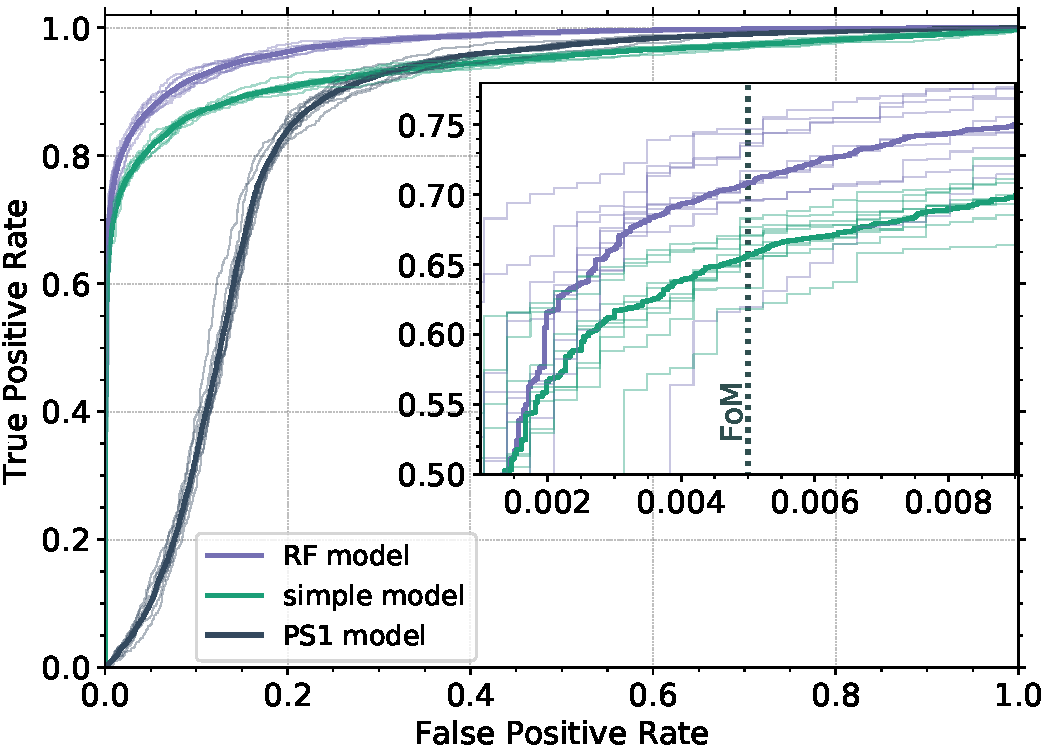
\includegraphics[width=3.35in, bb = 0 0 576 360]{./Figures/CV_ROC_HST.pdf}
  \caption{
  \NC{ ROC curves comparing the relative performance of the PS1, the simple, and the ML model. 
  We use PS1 sources cross-matched against the HST COSMOS catalog with 
  $\mathtt{iPSFMag} - \mathtt{iKronMag} \neq \mathrm{NaN}$ 
  so that any source in the dataset has a classification from all each model 
  for a fair comparison. 
  The solid orange, blue, and black line show the ROC curve 
  for the PS1 model, the simple model, and ML model, respectively. 
  Color-shadowed regions represent the standard deviation of each TPRs derived by 10-fold CV. 
  The ROC curves around FPR = 0.005 (grey solid line) are shown in the inset panel 
  (the ROC curve for the PS1 model is located at substantially below of the TPR range shown in the inset panel). 
  }
  }
  %
  \label{fig:cvroc_hst}
\end{figure}
%%%%%%%%%%%%%

Figure \ref{fig:cvroc_hst} shows the CV ROC curve of each models, 
and reveals the ML model is apparently outperformed to the other models. 
The overall ROC curve of the simple model, the new baseline of the performance of the star and galaxy separation, 
superiors to that of the PS1 model. 
The higher SNR of the difference between 
the \texttt{PSFFlux} and the \texttt{KronFlux} for each source 
in the simple model actually makes the performance of the classifier better, 
but the way to scoring to each object in this model, namely employing the distance from the threshold line, 
plays the most important role for this improvement, 
especially at the low FPR end (detail about the simple model, please see \S\ref{sec:simple_model}). 
In the simple model, a source difficult to judge whether it is star or galaxy ({\it i.e.,} a source at the faint end) 
has a score close to 0, 
while the source which can be distinguished clearly from a point source on the image 
has a large negative score (and vise versa for a point source). 
As most of stars do not have such large negative values, 
the lower FPR and the higher TPR is obtained at a large minus threshold for the star-galaxy classification. 
In the PS1 model, on the other hand, the classification is decided by $\mathtt{iPSFMag} - \mathtt{iKronMag}$, 
has an (essentially) identical score $\sim$0 for all stars independently of its distinguishability. 
The difference of the scoring method make substantial improvement of the performance of the PS1 model 
from that of the simple model at low FPR end. 

Since the ML model is trained with the 11 features 
consisting \texttt{whitepsfKronDist} and \texttt{whitepsfKronRatio}, 
which is the fundamental information for the classification in the  simple model and the PS1 model, respectively, 
the TPR of the ML model is higher than that of baseline models in whole FPR value. 
The ROC AUC is 0.973, 0.937, and 0.851, 
and the FoM is 0.715, 0.658, and 0.007, 
for the PS1 model, the simple model, and the ML model, respectively; 
in the other words, the TPR at the FPR$=0.5\%$ of the ML model and the simple model 
is improved 70.8$\%$ and 65.1$\%$ from that of the PS1 model, respectively. 

In Figure \ref{fig:cvacc_hst}, we compare the accuracy 
of the PS1 model, the simple model, and the ML model
evaluated via the PS1-HST data set as a function of \texttt{whiteKronMag}. 
%%% fig:cvacc_hst %%%
\begin{figure}[t]
 \centering
  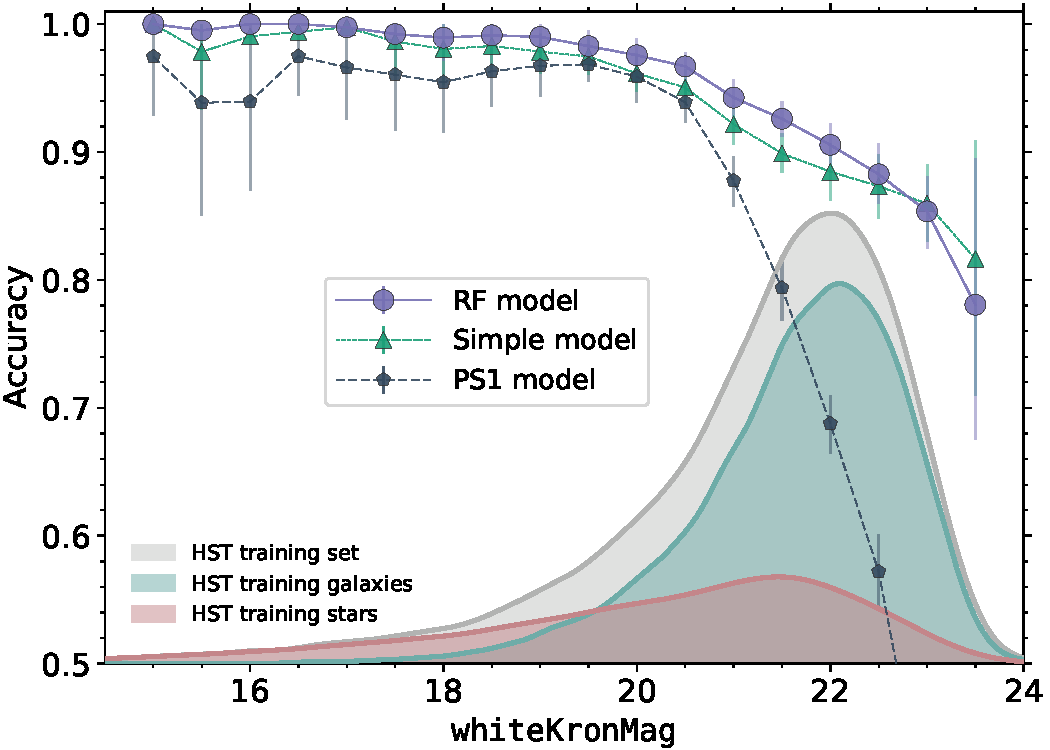
\includegraphics[width=3.35in, bb = 0 0 576 360]{./Figures/CV_Accuracy_HST.pdf}
  \caption{
  \NC{
  Predication accuracy of the PS1 model (orange filled circles), the simple model (blue filled circles), 
  and the ML model (black filled circles), as a function of \texttt{whiteKronMag} 
  for PS1 sources cross-matched against the HST COSMOS catalog. 
  Accuracies are shown in bin of width 0.5 mag, and the error bars 
  represents the range including 68\% of CV accuracies in each bin. 
  Additionally, a KDE of the PDF for stars and galaxies in the data set is shown in red and green, respectively. 
  The PDF of stars and galaxies has been normalized by the ratio of the number of stars and galaxies 
  to the full number of sources in the data set, respectively. 
  The KDE of the PDF for all sources in the dataset is also shown in grey.
  }
  }
  %
  \label{fig:cvacc_hst}
\end{figure}
%%%%%%%%%%%%%
In the PS1 model, prediction accuracy quickly decrease from $\mathtt{whiteKronMag} \sim $ 20 mag, 
to the level of random predictions (accuracy $\sim$ 0.5) for sources with $\mathtt{whiteKronMag} \gtrsim $ 23 mag. 
In the simple model, on the other hand, 
although is starting to decrease from $\mathtt{whiteKronMag} \sim $ 20 mag gradually to the faintest end, 
the accuracy is above 80\% even for sources fainter than $\mathtt{whiteKronMag} \sim $ 23.5 mag. 
This is mainly because higher SNR in ``white feature'' of the difference 
between \texttt{Kron} flux measurement and \texttt{PSF} flux measurement for each source (see \S\ref{sec:model_features}), 
differs to the case of the improvement of the ROC curve. 

The performance of the ML model is the best among other baseline models in almost all brightness of a source in the dataset, 
but one notice to the similarity of the accuracy curve of the ML model and the simple model. 
This is because of the highest importance of the \texttt{whitepsfKronDist} 
among all of 11 features for the classification of ML model. 
The overall CV accuracy of the ML model, the simple model, and the PS1 model is 
***, ***, and ***. 
As previously mentioned, the ML model provides superior predictions 
especially for faint sources, which will enable to us to best identify stars in ZTF survey imaging 
even outside the COSMOS field. 
Figure \ref{fig:cvacc_hst} also shows a KDE of the PSD of stars and galaxies in the PS1-HST data set 
as a function of \texttt{whiteKronMag}. 
The KDEs indicate that most of sources brighter than $\mathtt{whiteKronmag} \lesssim 19$ is star, 
while the number of galaxies overwhelms that of stars from $\mathtt{whiteKronmag} \gtrsim 21$ to the faintest end. 
The KDE of PDF for stars and galaxies has a peak around $\mathtt{whiteKronMag} \sim 21.5$ and $\sim 22$, 
respectively. 
We note that such distribution should be quite low-biased for the PS1 catalog 
since all of the sources in the catalog are taken from imaging data sets. 

\subsection{ML Comparison with SDSS photo}
%%% fig:roc_sdss %%%
\begin{figure}[t]
 \centering
  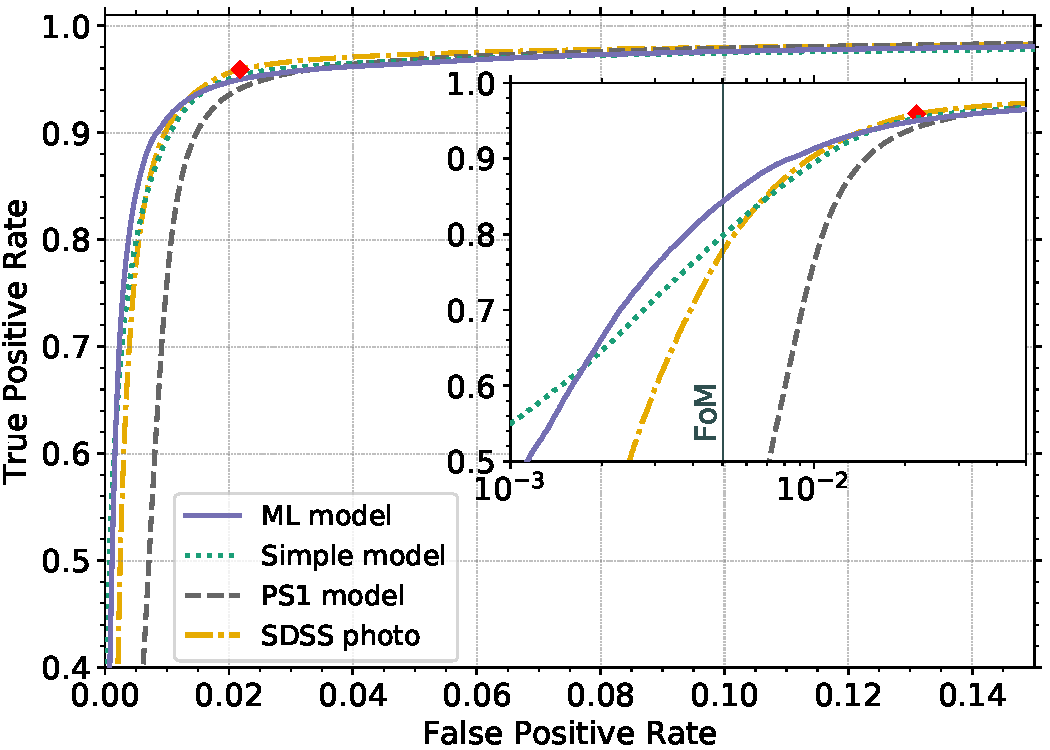
\includegraphics[width=3.35in, bb = 0 0 576 360]{./Figures/ROC_curves.pdf}
  \caption{
  \NC{
  ROC curves comparing the relative performance 
  of the SDSS photo model (green solid line), the PS1 model (orange solid line), 
  the simple model (blue solid line), and the Ml model (black solid line) 
  for PS1 sources cross-matched against the SDSS spectroscopic catalog. 
  The SDSS photometric classifier is shown as a red star on the ROC curve of the SDSS photo model, 
  due to the binary nature of the SDSS photometric classification. 
  The inset panel shows ROC curves around the FPR = 0.005 (grey solid line). 
  }
  }
  %
  \label{fig:roc_sdss}
\end{figure}
%%%%%%%%%%%%%
Next, we assess the performance of ML model by comparing with SDSS photometric classification 
by using PS1-SDSS spectroscopic catalog. 
Figure \ref{fig:roc_sdss} shows the ROC curve for 
the SDSS photo, the PS1 model, the simple model, and the ML model, 
by comparing predictions with SDSS spectroscopic classifications, 
which is independent with the training data set; PS1-HST cross-matched catalog. 
For sources in PS1-SDSS catalog, broadly, 
the performance of classifications by each model is better than that for sources in PS1-HST catalog. 
This is simply because that the distribution of sources, especially galaxies, in PS1-SDSS catalog 
are biased toward to brighter side comparing with of PS1-HST catalog. 
The selection bias of the SDSS spectroscopic survey 
toward observing luminous red galaxies (LRGs; {\it e.g.,} see \citealt{Eisenstein01}) 
results in the KDE of the PDF of galaxies having two peaks 
at $\mathtt{whiteKronMag} \sim 17$ and $\sim 20$ 
(see \S\ref{sec:sdss} and the left panel in Figure \ref{fig:acc_sdss}). 
As we alluded to in \S\ref{sec:comp_hst}, 
the distribution of stars and galaxies in the real universe (except the galactic plane) 
should be similar to that shown in Figure \ref{fig:cvacc_hst}; 
the peak of the distribution for stars and galaxies is around $\mathtt{whiteKronMag} \sim 22$ 
and the number of stars and of galaxies is dominant at the bright end and the faint end, 
respectively \citep{Chambers16}. 
Although the data set has the selection bias as mentioned above 
and thus the distribution of stars and galaxies as a function of brightness is totally different to that of the training set, 
the ROC curve of ML model is superior to the other models in terms of the FoM and also the ROC AUC; 
the FoM for the SDSS model, the PS1 model, the simple model, and the ML model is 
0.777, 0.290, 0.798, and 0.843, respectively, 
and the ROC AUC score for each model is 
0.987, 0.984, 0.985, and 0.987, respectively. 

%%% fig:acc_sdss %%%
\begin{figure*}[t]
 \centering
  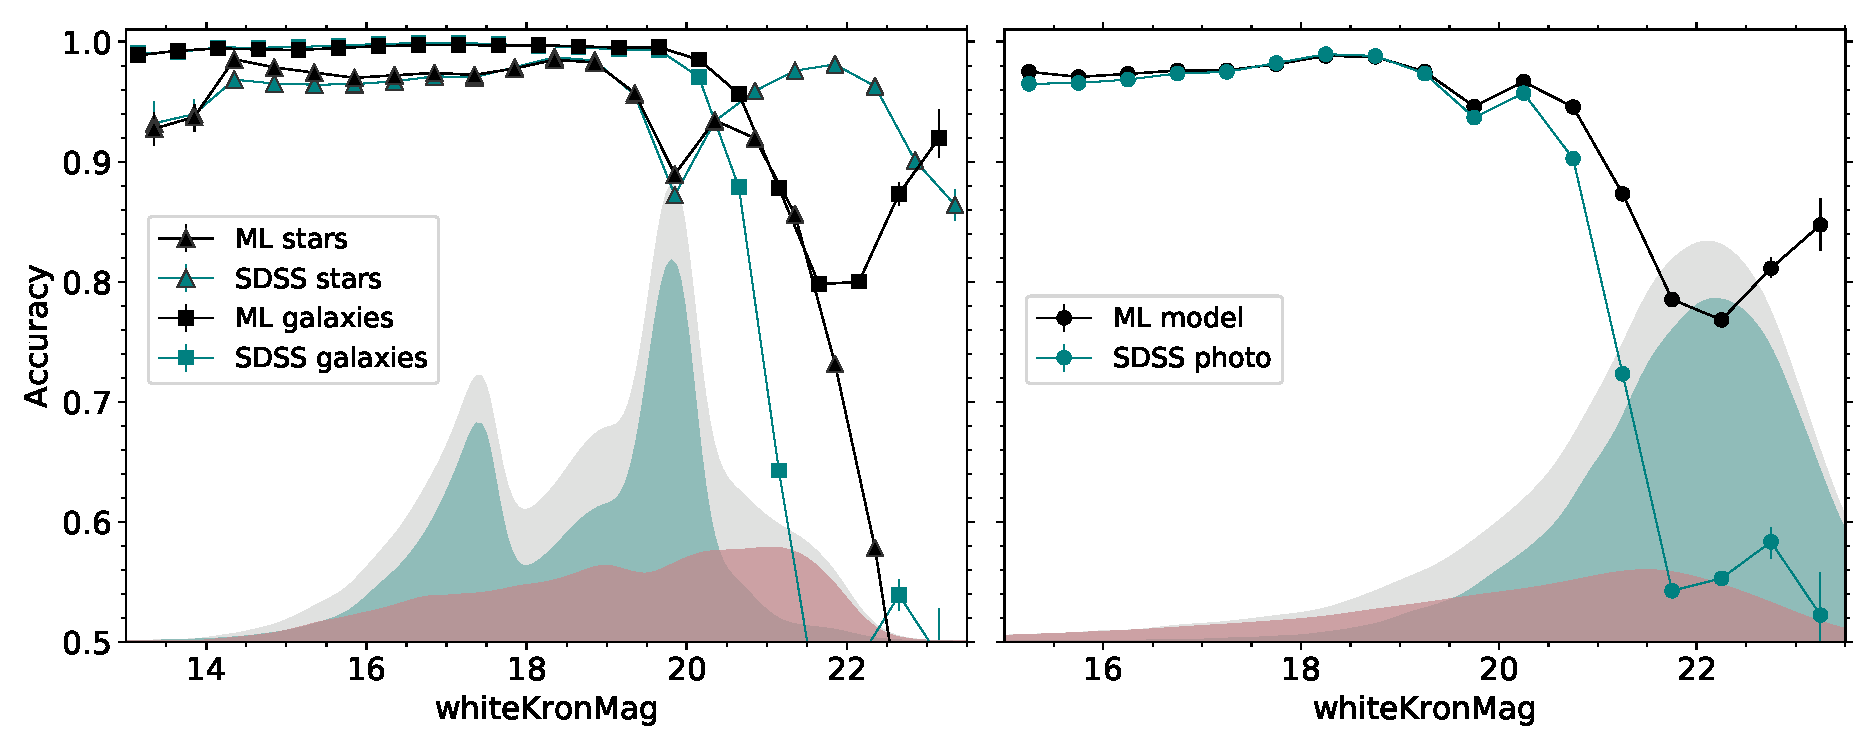
\includegraphics[width=6.5in, bb = 0 0 900 360]{./Figures/Accuracy_SDSS_ML_model.pdf}
  \caption{
  \NC{ 
  Prediction accuracy of the SDSS photo model and the ML model 
  as a function of \texttt{whiteKronmag} for PS1 sources cross-matched against the SDSS spectroscopic catalog. 
  In the left panel, the green filled square and the green filled triangle 
  show the prediction accuracy of the SDSS photo model for galaxies and stars, respectively, 
  and the black filled square and the black filled triangle show that of the ML model for galaxies and stars, respectively. 
  Accuracies are calculated in each 0.5 mag bin. 
  The KDE of the normalized PDF of stars and galaxies 
  in the PS1-SDSS cross-matched catalog is also shown in red and green, respectively (same way as Fig. \ref{fig:cvacc_hst}). 
  In the right panel, the overall accuracy of the SDSS photo model and the ML model 
  as a function of \texttt{whiteKronMag} is shown by filled green circle and filled black circle, respectively. 
  The accuracy in each bin is calculated for stars and galaxies picked up 
  from PS1-SDSS cross-matched catalog 
  so that the ratio the number of stars and galaxies in each bin is 
  same with that in the PS1-HST cross-matched catalog. 
  The KDE of PDF of stars and galaxies in PS1-HST cross-matched catalog is shown in red and green, respectively. 
  }
  } 
  %
  \label{fig:acc_sdss}
\end{figure*}
%%%%%%%%%%%%%
In the left panel of Figure \ref{fig:roc_sdss}, we show the prediction accuracy of the SDSS photo model 
and the ML model for galaxies and stars separately. 
One can see that an unusual systematic whereby a large fraction of stars with $\mathtt{whiteKronMag} \sim 20$ 
were erroneously classified as galaxies by both of models. 
The reason of it is discussed by \cite{Miller17}; 
red stars blended with fainter sources would be classified to be galaxies. 
Interestingly, for the SDSS photo model, the accuracy for galaxies is rapidly decreasing from \texttt{whiteKronMag}, 
while that for stars stays above $\sim 0.9$. 
It means the SDSS photo model is optimized to separate stars and galaxies in the SDSS spectroscopic catalog, 
namely, the model classifies most of faint sources as stars 
since the number of stars overwhelms that of galaxies from $\sim 21$ mag to the faint end in this catalog. 

For evaluating the performance of the SDSS photo model and the ML model 
for the star/galaxy population similar to the real universe, 
we calculate the prediction accuracy of each model in a different way; 
we pick up sources from PS1-SDSS catalog 
so that the ratio of the number of stars and to the number of galaxies 
is same as that in PS1-HST catalog, and then calculate the prediction accuracy of each model in each 0.5 mag bin. 
The result is shown in the right panel of Figure \ref{fig:acc_sdss}. 
The prediction accuracies shows that the performance of each model is similar 
down to $\mathtt{whiteKronMag} \sim20.5$, 
while the performance of the SDSS photo model quickly degrades for fainter sources. 
This is to be expected based on the poor performance for faint galaxies of the SDSS photo model; 
the PS1-HST catalog (and also the real universe) contains much large number of faint galaxies than faint stars. 
The final ML model, which is optimized to classify stars and galaxies following this population, 
will provide the most accurate classification for sources in high-latitude sky. 
} 






\section{Discussion}

\section{The PS1 Catalog Deployed: Integration in ZTF}

\todo{provide a description for how the catalog is used by ZTF in real-time ops}

\section{Conclusions}

\acknowledgements

\begin{itemize}
    \item Brian Bue (possibly also Umaa, check emails)
    \item PS1 casjobs (Bernie in particular)
\end{itemize}

AAM is funded by the Large Synoptic Survey Telescope Corporation in support of
the Data Science Fellowship Program. 
Y.T. is funded by JSPS KAKENHI Grant Numbers JP16J05742. 

\facility{PS1}

\software{\texttt{astropy} \citep{Astropy-Collaboration13}, 
          \texttt{scipy} \citep{Jones01}, 
          \texttt{matplotlib} \citep{Hunter07},
          \texttt{pandas} \citep{McKinney10}}


\appendix


\bibliographystyle{aasjournal}
\bibliography{star_gal}

\end{document}